%----------------------------------------------------------------------------------------
%	Data Structures
%----------------------------------------------------------------------------------------
\section{Data Structures}

%------------------------------------------------
%Subsection: Java basics
\subsection{Java Basics}

In Java, there are \textbf{primitive types} and \textbf{reference types}. Primitive types are like \texttt{short}, \texttt{int}, \texttt{long}, \texttt{float}, \texttt{double}, \texttt{boolean}, \texttt{char}, \texttt{byte}. Reference types are \textbf{arrays} and \textbf{classes}. 

When you declare a variable with a reference type, you get space for a reference or \textbf{pointer} to that type, not for the type itself. Use \texttt{new} to get space for the type itself. Non-primitive types are really pointers. Assigning 1 variable to another can cause \textbf{aliasing} (two or more different names reference the same object). 

For each \textbf{primitive type} there is a "box class" or "wrapper class". For instance, the \texttt{Integer} class contains one \texttt{int} value. Java \textbf{autoboxing} converts between the primitive and wrapper classes as appropriate. 

Java also has \textbf{visibility modifiers}, which specify how code can be accessed.
\begin{itemize}
	\item \textit{public} accessible to any code
	\item \textit{private} accessible to code within same class
	\item \textit{protected} accessible to code within same class or subclasses
	\item \textit{public} accessible to code within same package (directory)
\end{itemize}

Numerical comparisons can be performed using the "<", ">", "=" signs for \texttt{int}, \texttt{float}, \texttt{double} primitives. However, the \textbf{Comparable} interface should be used for objects in Java (\texttt{String}, \texttt{Integer}, \texttt{Double}). The \texttt{compareTo} method returns negative value if "less than", zero if "equal to", and positive if "greater than". 

%------------------------------------------------
%Subsection: Complexity
\subsection{Complexity}

Complexity is a way to gauge the performance of an algorithm: how much of the computing resources are used when a program executes. \textbf{Complexity} measures how the resource requirements scale as the problem gets larger. The time requirement is basically proportional to the number of basic operations such as '+', '*', one assignment, one logical test, one read, or one write. The \textbf{problem size} is related to the number of important factors. In sorting, for example, this could be the number of elements to sort. 

We are usually interested in the worst case number of operations, not the exact number of operations, which can vary. The average and best cases do provide useful information, however. We use the \textit{big-O} notation to write complexity: $O(N)$ is linear complexity, $O(N^{2})$ is quadratic complexity, etc. 

%------------------------------------------------
%Subsection: ADTs
\subsection{Abstract Data Types}

Abstract Data Types (\textbf{ADTs}) separate the \textit{specification} of a data structure from the \textit{implementation} of that data structure. The specification refers to the methods and operations that can be performed on it, while the implementation refers to how those features are programmed. The advantage to using ADTs is that code is more reusable: the implementation of certain code can be changed without changing the programs that use the code. An ADT corresponds to a class or many implementing classes. Operations on an ADT are the class's \textbf{public methods}. Example operations on an ADT include: initialize, add data, access data, remove data.

ADTs have 2 parts.
\begin{itemize}
	\item public/external - conceptual picture \& conceptual operations
	\item private/internal - the representation (how the structure is stored) and the implementation of operations (code)
\end{itemize}

To implement an interface in Java: (1) include "\texttt{implements InterfaceName}" in the class declaration, changing \texttt{InterfaceName} as appropriate, (2) define a public method for the class for each method signature in the interface. 

To specify that something is a subclass, use \texttt{extends}. This says that the current class definition inherits from the specified class. For instance, \texttt{MyException} inherits from the \texttt{Exception} class in the example below. \\

\texttt{public class MyException extends Exception \{...\};} \\

%------------------------------------------------
%Subsection: Exceptions:
\subsection{Exceptions}

Errors can arise due to \textit{user error} (e.g. wrong inputs) or \textit{programmer error} (e.g. buggy code). It is desirable to pass the error up from low-level methods to a level where it can be handled properly. In C++, methods usually just return a special value to indicate an error. Requires calling code to check for error. In Java, expections allow error testing in the code. 

The idea is to \textbf{throw} an \textbf{exception} when an error is detected. The code causing the error stops executing immediately and control is transferred to the \textbf{catch clause} for that type of exception of the first enclosing \textbf{try block} that has such a clause. The try block might be in the current method or in a method that called the current one. The exception is passed up the call chain, all the way up to \texttt{main} or the Java virtual machine if necessary (at which point the program stops and an error message appears). The code below provides an example. \\ 

\texttt{try \{} \\
\indent \indent \texttt{// code that might cause exceptions.} \\
\indent \texttt{\} catch( ExceptionType1 id1 ) \{} \\
\indent \indent \texttt{// statement to handle this exception type.} \\
\indent \texttt{\} catch( ExceptionType2 id2 ) \{} \\
\indent \indent \texttt{// statement to handle this exception type.} \\
\indent \texttt{\} finally \{} \\
\indent \indent \texttt{// statement to execute every time this try block executes.} \\
\indent \texttt{\}} \\

Each \texttt{catch} clause specifies one type of exception and provides a name for it, like method objects. The \texttt{finally} clause is optional. It \textit{always} executes if the \texttt{try} block is entered. Note: you can have zero catch clauses and still have a finally clause. 

Java's standard libraries have several built-in exceptions: \texttt{ArithmeticException}, \texttt{ClassCastException}, \texttt{IndexOutOfBoundsException}, \texttt{NullPointerException}, \texttt{FileNotFoundException}...

All exceptions are either \textbf{checked exceptions} or \textbf{unchecked exceptions}. If a method includes code that could cause a checked exception to be thrown: (1) the exception must be declared in the method header using a \textbf{throws} clause, or (2) the code that might cause the exception to be thrown must be in a try block with a catch clause for that exception. Otherwise you will get a compiler error. Unchecked exceptions do not need to be listed in the throws clause of a method. The code below provides an example. \\

\texttt{public static void main( string[] args ) throws FileNotFoundException, EOFException \{} \\
\indent \indent \texttt{// those two exceptions might be thrown here.} \\
\indent \texttt{\}} \\

Unchecked exceptions are subclasses of \texttt{RuntimeException}, while checked exceptions are subclasses of \texttt{Exception} only, not \texttt{RuntimeException}. Most built-in Java exceptions are unchecked, with the exception of I/O exceptions, which are checked. user defined exceptions should usually be checked. 

Java exceptions are objects, and as such a new exception is made by defining a new instantiable class. It must be a subclass of \texttt{Throwable}, usually a subclass of \texttt{Exception}. An example is given below. \\

\texttt{public class EmptyStackException extends Exception \{} \\
\indent \indent \texttt{public EmptyStackException() \{ super(); \}} \\
\indent \indent \texttt{public EmptyStackException(string message) \{ super(message); \}} \\
\indent \texttt{\};} \\


At the point in code where an error is detected, the exception is thrown using a \texttt{throw} statement. \\

\texttt{if (...) \{ throw new EmptyStackException(); \}} \\

%------------------------------------------------
%Subsection: List Structure
\subsection{List Structure}
\subsubsection{Basic List}
A \textbf{List} structure is an ordered collection of items of some element type \textit{E}. One advantage of lists over arrays is that they are variable size. A disadvantage is that you cannot have an empty list with non-zero size. Lists only hold objects, whereas arrays hold any type (even primitive types such as \texttt{int}, \texttt{char}). 

The table below provides the public interface for the \texttt{ListADT}. \\

\begin{tabular}{p{0.4\textwidth}p{0.6\textwidth}}
\texttt{void add(int pos, E item);} & Add an item at a specified position \\
\texttt{void add(E item);} & Append item to end of list \\
\texttt{boolean contains(E item);} & Check if list contains item \\
\texttt{int size();} & Get the number of items in the list \\ 
\texttt{boolean isEmpty();} & Check if list contains zero items \\
\texttt{E get(int pos);} & Get the item at the specified position \\
\texttt{E remove(int pos);} & Remove, return item at specified pos. \\
\end{tabular} \\

To instantiate \texttt{ListADT}, for a list of \texttt{Integer} type items named \texttt{number} using the \texttt{ArrayList} class: \\

\texttt{ListADT<Integer> numbers = new ArrayList<Integer>();}. \\

\texttt{\textbf{Iterator}} is a defined interface in \texttt{java.util}. Iterating accesses each item in a list in turn. The interface is \texttt{Iterable}. Every java class that implements Iterable (from \texttt{java.lang} provides an \texttt{iterator} method that returns an \texttt{Iterator} object for that collection. For example, the \texttt{List<E>} interface has an \texttt{iterator()} method: \\

\texttt{Iterator<string> itr = words.iterator(); //words is a List<String>} \\

The easiest way to implement an iterator for a class is usually to define a new class. For example, in the \texttt{SimpleArrayList} class, the \texttt{iterator()} method should return a new \texttt{SimpleArrayListIterator} object. \\

Here's a simple overview of an iterator class: \\

\texttt{import java.util.Iterator;} \\
\indent \texttt{import java.util.NoSuchElementException;} \\
\indent \texttt{public class SimpleArrayListIterator implements Iterator<Object> \{} \\
\indent \indent \texttt{// methods:} \\
\indent \indent \texttt{public boolean hasNext()\{...\}} \\
\indent \indent \texttt{public Object next()\{...\}} \\
\indent \indent \texttt{public void remove()\{...\}} \\
\indent \texttt{\};} \\

\subsubsection{Linked Lists}

\textbf{Linked lists} are a type of list in which each item in the list contains the item data as well as a reference to the next element in the list. The list is built using \texttt{Listnode} objects that store data as well as the next listnode. The \texttt{getNext()} method returns the next item in the list, which can also be set using the \texttt{setNext(Listnode<E> n)} method. 

Linked lists often have a \textbf{header node} -- a dummy node at the front of the list. Header nodes do NOT contain data, the only include a reference for the next item. A \textbf{tail pointer} references the last listnode. 

There are many variants of linked lists, including doubly linked lists (which have a reference to the previous and next elements) and circularly linked lists (where the tail node \texttt{next} is linked to the first node). 

%------------------------------------------------
% Subsection: Queue and Stack
\subsection{Stacks and Queues}

Stacks and queues are like lists, but with more limited operations. They can be implemented using an array or linked list. 

\subsubsection{Stacks}

A \textbf{stack} is a stack of items. Only the top item can be accessed. Items are added to the top of a stack. It is a basic \textbf{LIFO} structure: a last-in-first-out data type. A basic stack interface is provided below. \\

\texttt{public interface StackADT<E> \{} \\
\indent \indent \texttt{boolean isEmty(); //return true iff empty} \\
\indent \indent \texttt{void push(E obj); // add object to top of stack} \\
\indent \indent \texttt{E pop() throws EmptyStackException; //remove} \\
\indent \indent \texttt{E peek() throws EmptyStackException; // see} \\
\indent \texttt{\};} \\

\subsubsection{Queue}

A \textbf{queue} is a structure similar to a line or queue. Items go in one side and out the other. It is a basic \textbf{FIFO} structure: a first-in-first-out data type. Items are added to the \textit{rear} of the queue and removed from the \textit{front} of the queue. \\

\texttt{public interface QueueADT<E> \{} \\
\indent \indent \texttt{boolean isEmty(); //return true iff empty} \\
\indent \indent \texttt{void enqueue(E obj); // add object to end of queue} \\
\indent \indent \texttt{E dequeue() throws EmptyQueueException; //remove from front} \\
\indent \texttt{\};} \\

%------------------------------------------------
% Subsection: Recursion
\subsection{Recursion}

A method is \textbf{recursive} if it can call itself either directly or indirectly. Recursive code is often \textit{simpler}, but not faster or more efficient. There are a few rules associated with recursion. 

\begin{itemize}
	\item \textit{Recursion rule 1}: recursive methods must have a \textbf{base case} - a condition under which no recursive call is made. This prevents infinite recursion. 
	\item \textit{Recursion rule 2}: every recursive method \textbf{make progress} towards a base case. 
\end{itemize}

At runtime, a stack of activation records (AR) is maintained (one for each active method). This is also named the \textbf{call stack}. It includes the method's parameters, local variables, and return address. When a method is called, its AR is pushed onto the stack. When too many methods are called, a \textbf{stack overflow} error is produced. 

A data structure is recursive if it can be defined in terms of itself. 

%------------------------------------------------
% Subsection: Searching
\subsection{Searching in an Array}

There are two basic approaches to searching in an array: \textbf{sequential} search and \textbf{binary} search. Sequential search involves looking at each value in turn. It is faster for sorted arrays $O(N)$. Binary search (for sorted array) involves looking at the middle item, comparing with the value of interest, then eliminating half of the array from the search $O(\log(N))$. 

%------------------------------------------------
% Subsection: Tree Structure
\subsection{Tree Structure}

So far, the structures discussed have been \textbf{linear data structures}. These incude lists, stacks, queues, and other structures in which items are stored with one item following another. \textbf{Trees} are an example of a \textbf{nonlinear data structure}. More than one item can follow from a single item. Furthermore, the number of following items can vary from one item to another. Trees are useful because they can provide \textit{fast access} to information in a database. 

Some tree terminology is provided in the table below. \\


\begin{tabular}{p{0.3\textwidth}p{0.7\textwidth}}
\textbf{Node} & A single element of the tree \\
\textbf{Edge} & Arrow connecting two nodes \\
\textbf{Root} & Top-most node of the tree (has no \textbf{parent}) \\
\textbf{Leaf} & bottom nodes (has no \textbf{children}) \\
\textbf{Ancestors} & The preceding nodes in a tree \\
\textbf{Descendants} & The succeeding nodes in the tree \\
\textbf{Path} & A sequence of conected nodes \\
\textbf{Path Length} & Number of nodes in the path \\
\textbf{Height} & Length of \textit{longest} path from root to a leaf \\
\textbf{Depth} & Path length from a given node back to root \\
\end{tabular} \\

\subsubsection{Binary Trees}

\textbf{Binary trees} are a special type of tree in which (1) each node has 0, 1, or 2 children and (2) each child is either a \textit{right} or \textit{left} child. 

Programming a binary tree usually requires a tree class and a tree node class. The \texttt{BinaryTreenode} class only requires 3 fields: \texttt{data}, \texttt{leftChild}, and \texttt{rightChild}. A generic tree, by comparison, could just use a list of nodes for the children. 

There are several ways to traverse a tree, as shown in the table below. V=view/visit, L=go to left child, R=go to right child. \\

\begin{tabular}{p{0.2\textwidth}p{0.5\textwidth}p{0.2\textwidth}}
\textit{Name} & \textit{for binary tree} & \textit{for other tree} \\
\hline
\textbf{pre-order} & VLR & VC \\
\textbf{post-order} & LRV & CV \\
\textbf{level-order} & left to right from top to bottom \\
\textbf{in-order} & LVR & (binary only) \\
\end{tabular} \\

\subsubsection{Binary Search Trees}

A \textbf{binary search tree} (BST) is a type of binary tree that stores sorted values. For every node \textit{n} with a \textbf{key value} (and maybe data):

\begin{itemize}
	\item all keys in \textit{n}'s left sub-tree are less than the key in \textit{n},
	\item all keys in \textit{n}'s right sub-tree are greater than the key in \textit{n}.
\end{itemize}

A binary search tree has efficient implementations of the insert, contains, remove, and print methods. Example structures for the node and tree classes are provided below. \\

\texttt{class BSTnode<K> \{} \\
\indent \indent \texttt{private K key;} \\
\indent \indent \texttt{private BSTnode<K> left, right;} \\
\indent \indent \texttt{public BSTnode(K key, BSTnode<K> left, BSTnode<K> right) \{...\} }; \\
\indent \indent \texttt{//accessors:} \\
\indent \indent \texttt{public K getKey()\{...\}} \\
\indent \indent \texttt{public BSTnode<K> getLeft()\{...\}} \\
\indent \indent \texttt{public BSTnode<K> getRight()\{...\}} \\
\indent \indent \texttt{//mutators:} \\
\indent \indent \texttt{void setKey(K key)\{...\}} \\
\indent \indent \texttt{void setLeft(BSTnode<K> left)\{...\}} \\
\indent \indent \texttt{void setRight(BSTnode<K> right)\{...\}} \\
\indent \texttt{\};} \\

\texttt{public class BST<K extends Comparable<K> > \{} \\
\indent \indent \texttt{private BSTnode<K> root;// root of BST} \\
\indent \indent \texttt{public void insert(K key)\{...\}} \\
\indent \indent \texttt{public void delete(K key)\{...\}} \\
\indent \indent \texttt{public boolean lookup(K key)\{...\}} \\
\indent \indent \texttt{public void print(PrintStream p)\{...\}} \\
\indent \texttt{\};} \\

Of course, it is also possible to design a BST that stores data along with each key. 

The l\texttt{ookup(K key)} method is an example of a recursive algorithm. The base cases are an empty tree, which returns false, or value is in the root node, which returns true. Check the root, left, and right subtrees. The worst-case lookup for a BST is $O(N)$, and corresponds to a stalky shape. Best case performance for a BST lookup is $O(\log(N))$ for a full, balanced tree. 

Question: how do you \textbf{delete} a node in a tree with children? And with what do you replace the deleted node? Possibilities:
\begin{itemize}
	\item the largest value in the left subtree (\textbf{in-order predecessor}). 
	\item the smallest value in the right subtree (\textbf{in-order successor}). 
\end{itemize}

The Java standard library implements a BST with the \texttt{TreeSet} and \texttt{HashSet} classes. Use \texttt{Map} and \texttt{TreeMap} to associate data with each key. 

A few additional tree types are listed below.

\begin{itemize} 
	\item \textbf{Full tree}: all the leaves have the same depth. 
	\item \textbf{Complete tree}: full to depth H-1, depth H filled from left to right. 
	\item \textbf{Height-balanced tree}: difference in heights of \textit{left} and \textit{right} subtrees is at most 1. 
	\item \textbf{Balanced tree}: has a height of $O(\log(N))$, where $N$=\# nodes.
\end{itemize}

\subsubsection{Red-Black Trees}

\begin{figure}[tb]
\centering
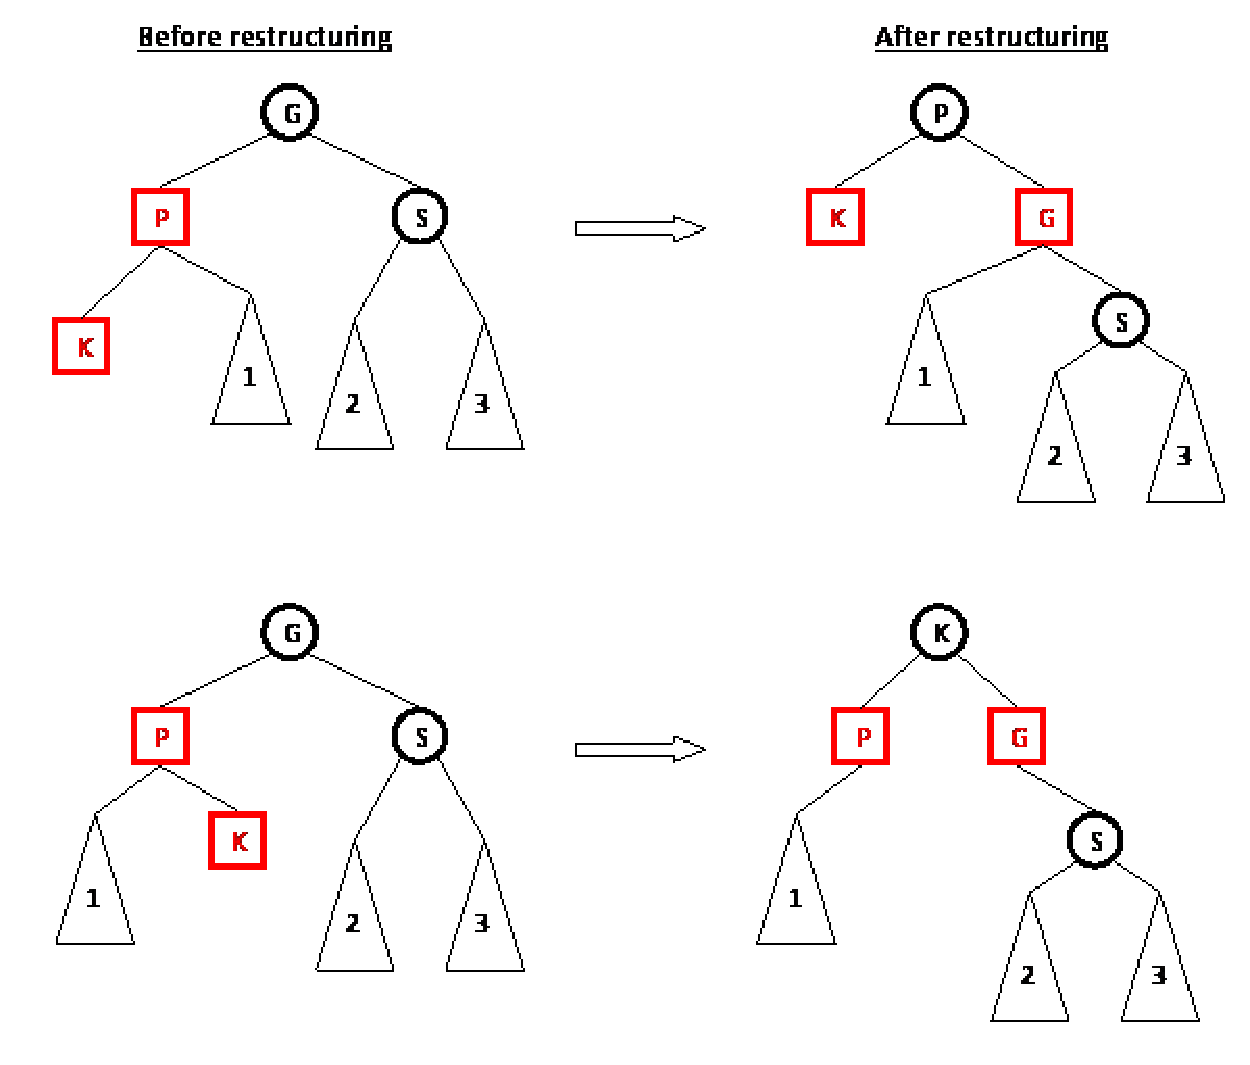
\includegraphics[width=0.75\columnwidth]{Figures/restructure.pdf}
\caption{An example of a \textbf{tri-node restructuring} procedure for a red-black tree (c.o. James D. Skrentny, University of Wisconsin CS367).}
\label{fig:trinoderestructuring}
\end{figure}

\begin{figure}[tb]
\centering
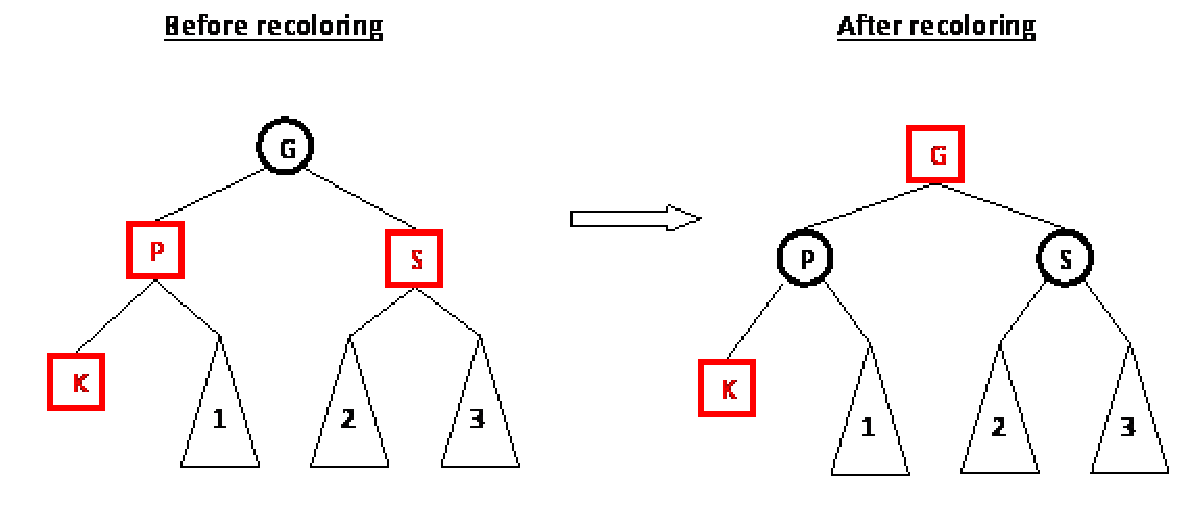
\includegraphics[width=0.75\columnwidth]{Figures/recoloring.pdf}
\caption{An example of a \textbf{recoloring} procedure for a red-black tree (c.o. James D. Skrentny, University of Wisconsin CS367).}
\label{fig:recoloring}
\end{figure}

\textbf{Red-black trees} (RBT) are a type of balanced tree. In order to preserve balance, the \texttt{insert} and \texttt{delete} operations may restructure the tree. Each node of the tree has a \textbf{color} (red or black), and 3 properties hold:

\begin{itemize}
	\item \textbf{Root property}: the root of the tree is black.
	\item \textbf{Red property}: children of a red node are black. 
	\item \textbf{Black property}: for each node with at least 1 null child, the number of black nodes on the path from the root to the null child is the same. 
\end{itemize}

We want to perform insert, lookup, delete, and print operations on this tree. Lookup and print for the RBT are identical to those of the BST. The lookup, insert, delete operations have $O(\log(N))$ complexity for the worst-case. 

Here's an overview of the RBT insert algorithm for node with key K. 

\begin{itemize}
	\item Use the BST insert algorithm to add K to the tree.
	\item Color the node containing K \textbf{red}.
	\item Restore the RBT properties if necessary.
\end{itemize}

Insertion can lead to a red property violation \textbf{RPV}. Here's how to deal with that. 

\begin{itemize}
	\item \textit{Case 1}: if K's parent P is black, then do nothing (no RPV). 
	\item \textit{Case 2a}: if P's sibling is black or null, do a \textbf{trinode restructuring}. 
	\item \textit{Case 2b}: if P's sibling S is red, do a \textbf{recoloring} of P, S, G (unless G is the root). 
\end{itemize}

\subsubsection{Balanced Search Trees}

There are other types of search trees that preserve the $O(\log(N))$ tree height that produces efficient operations for $N$ nodes. Other than red-black trees there are also AVL and BTree objects. 

An \textbf{AVL} is a height-balanced binary search tree. It was the first such structure to be invented, and is named after its Soviet inventors. 
\begin{itemize}
	\item Keeps a balance value for each node (-1, 0, +1).
	\item Detect problem when balance becomes $\pm 2$. 
	\item Fix by \textbf{rotation}. 
\end{itemize}

\begin{figure}[tb]
\centering
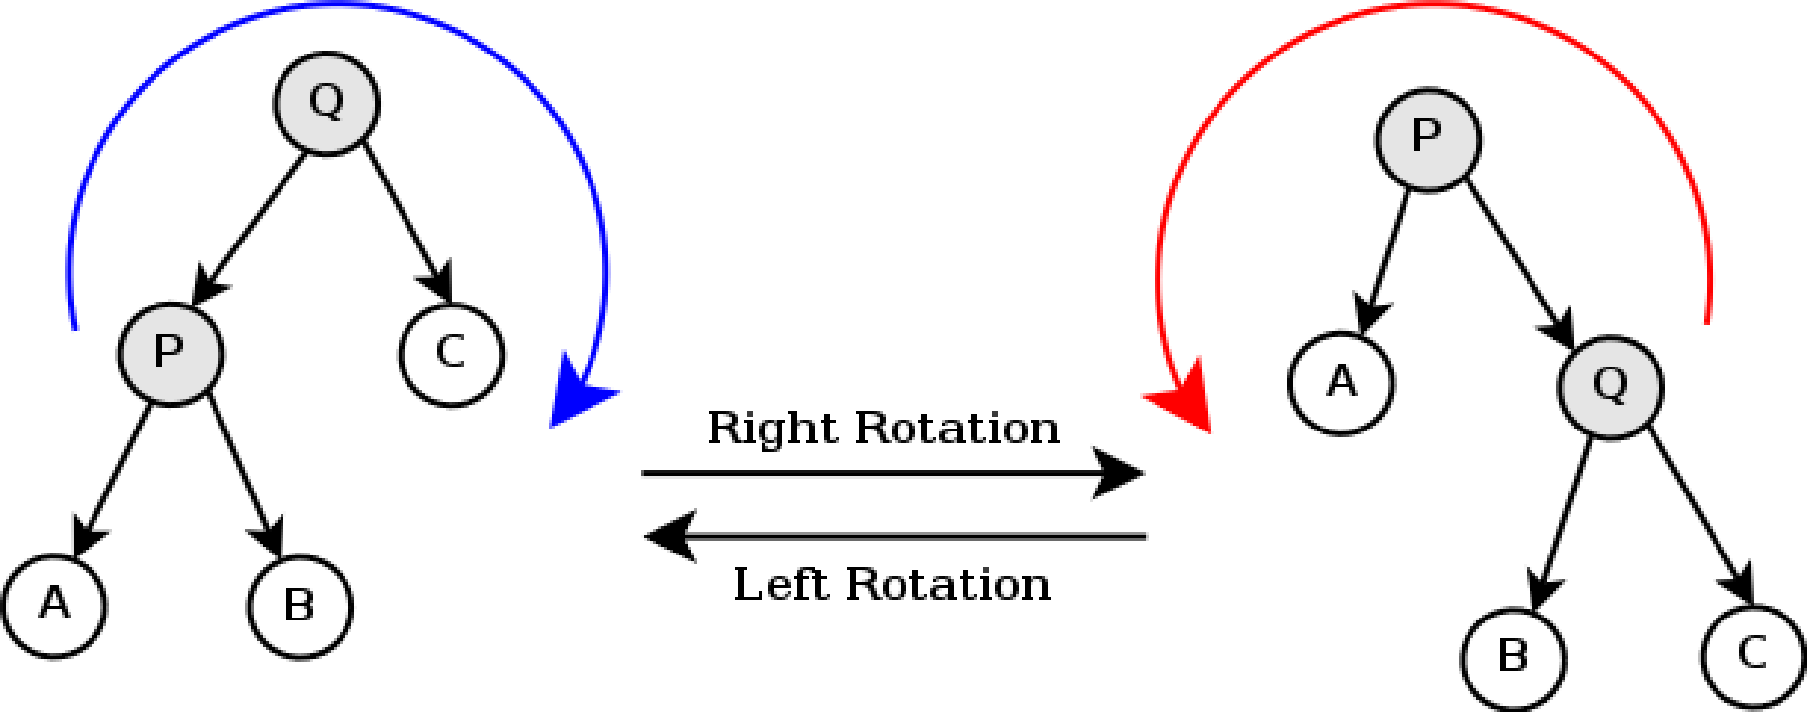
\includegraphics[width=0.75\columnwidth]{Figures/Tree_rotation.pdf}
\caption{An example of a tree rotation (By Ramasamy at the English language Wikipedia, CC BY-SA 3.0, https://commons.wikimedia.org/w/index.php?curid=4043513).}
\label{fig:rotation}
\end{figure}

\textbf{BTrees} relax the binary tree structure by allowing 2, 3, 4 descendant nodes (the number of allowed nodes is called the order). BTrees are also referred to sometimes as 2-3 trees or 2-3-4 trees. When 4 nodes are detected, they are split. 

%------------------------------------------------
% Subsection: Priority Queues
\subsection{Priority Queues}

\textbf{Priority queues} are a data structure where priorities are put into the object and highest priorities are removed from the object. Here are the basic priority queue operations:

\indent \indent \texttt{boolean isEmpty()} \\
\indent \indent \texttt{void insert(Comparable p);} \\
\indent \indent \texttt{void insert(Comparable p);} \\
\indent \indent \texttt{Comparable removeMax();} \\
\indent \indent \texttt{Comparable getMax();} \\

To implement the priority queue efficiently, a new data structure called a heap will be implemented. A \textbf{heap} is a binary tree with two special properties.

\begin{itemize}
	\item \textbf{Order property} for every node N, the value N is greater than or equal to the values in its children. 
	\item \textbf{Shape property} 
	\begin{itemize}
		\item All leaves are at depth $d$ or $(d-1)$.
		\item All of the leaves at depth $(d-1)$ are to the right of the leaves at depth $d$.
		\item There is at most 1 node with just 1 child. That child is the left child of its parent. It is the rightmost leaf at depth $d$. 
	\end{itemize}
\end{itemize}

The \textbf{root} of the heap is always in \texttt{array[1]}. If a node is in \texttt{array[k]}, the left child is in \texttt{array[2*k]}, the right child is in \texttt{array[2*k+1]}, and the parent is in \texttt{array[k/2]}.

Implementing \textbf{heap insert}:
\begin{itemize}
	\item add new value at the end of the array (preserve shape),
	\item swap with parent until order property holds, or get to root.
\end{itemize}

Implementing \textbf{heap removeMax}:
\begin{itemize}
	\item replace the value with the value at the end of the array (removing leaf), 
	\item work way down the tree, swapping value with the larger child to restore the order property.
\end{itemize}

The insert and remove operations described above are for a \textbf{max heap}. Of course, it is also possible to have a \textbf{min heap} along the same lines. 

%------------------------------------------------
% Subsection: Hashing
\subsection{Hashing}

\textbf{Hashing} is a technique that is $O(1)$ average complexity for insert, lookup, and delete operations. The basic idea is to store values (\textit{keys}) in an array, computing each key's position in the array as a function of its value. The array storing data is referred to as the \textbf{hash table}, while the function that maps keys to array indices is called the \textbf{hash function}. It is good to use efficient hash functions. For example, one can convert the key value to an integer modulo the table size. 

One issue that arises with hashing is that multiple data items might map to the same array index. \textbf{Collisions} occur when key values map to the same index. There are a few tricks that help to avoid collisions. First, it is best to use a table that is 1.25 times the size of the expected number of items and then to expand the hash table as necessary. Second, it is good to have a \textit{prime} table size, so that hashing functions that include multiplication by some factor don't send all keys to the same bucket after the hash function modulation. Ideally, you want the generator for the hash index to use a constant that is co-prime with the hash table length. 

\textbf{Buckets} are used to handle keys that get mapped to the same array index. \textit{LinkedList} buckets can be used for the buckets. This structure would give $O(1)$ complexity for insertion but $O(N)$ worst-case complexity for other operations. Another option would be to use a BST bucket, which would give $O(\log(N))$ worst-case complexity when all keys are mapped to one index.

Java has a \texttt{hashCode()} method for every Object, including \texttt{Strings}. 

Another way to handle collisions is through open addressing. If there is a collision, search for an unused element elsewhere in the table using a \textbf{probe sequence}. The list below uses $H$ to represent the hash function result for an item $k$:

\begin{itemize}
	\item \textit{linear probing}: $H(k), H(k)+1, H(k)+2, ...$ \% table size
	\item \textit{quadratic probing}: $H(k), (H(k)+1)^{2}, (H(k)+2)^{2}, ...$ \% table size
	\item \textit{double hashing}: $H(k), (H(k)+step), (H(k)+2\cdot step), ...$ \% table size
\end{itemize}

%------------------------------------------------
% Subsection: Graph Structure
\subsection{Graph Structure}

\textbf{Graphs} are a generalization of the tree structure. They have \textbf{nodes} connected by \textbf{edges} (also called \textit{vertices} or \textit{arcs}). A nide can have any number of incoming or outgoing edges. There are directed and undirected graphs.

\textbf{Undirected graphs} have nodes which are connected by edges without any direction. Connected (adjacent) nodes are simply referred to as \textbf{neighbors}. 

\textbf{Directed graphs} have neighbor nodes that are connected by edges with a \textbf{direction}. The source of the edge is referred to as the \textbf{predecessor} node, while the target of the edge is referred to as the \textbf{successor} node. 

\textbf{Paths} can be taken through the nodes in a graph. A \textit{cyclic path} is a path in which the same node occurs twice. An \textit{acyclic path} path is a path in which no node is repeated. Note: a node can connect an edge to itself. 

Here are some types of graphs:
\begin{itemize}
	\item \textit{directed acyclic graph (DAG)}: a directed graph that has NO cyclic paths. 
	\item \textit{Complete graph}: an undirected graph that has an edge between every pair of nodes, or a directed graph that has an edge from every node to every other node. 
	\item \textit{Weighted graph}: A graph with values associated with the edges. 
	\item Ptextit{Network}: A weighted di-graph (directed graph) with non-negative weights. 
\end{itemize}

\subsubsection{Depth-First Search}

A \textbf{depth-first search}, or DFS, is a method for searching through the nodes in a graph. It usually is implemented with a \textit{stack} or \textit{recursive} structure. The idea is to start at some node $n$, then follow an edge of of $n$, then another edge, getting as far away from $n$ as possible before visiting any more of $n$'s successors. 
\begin{itemize}
	\item start with all nodes marked "unvisited"
	\item mark $n$ "visited"
	\item recursively do a DFS from each of $n$'s unvisited successors. 
\end{itemize}

The time for this search is $O(N+E)$, where N=\# nodes and E=\# edges in the graph. A boolean in the node class could store visited information.

There are many applications of the depth-first search. It can answer questions like the following.
\begin{itemize}
	\item Is a graph connected?
	\item Does the graph contain a cycle?
	\item Is there a path between two nodes?
	\item What nodes are reachable from the given node?
	\item Can the nodes be ordered so that, for every node $j$, $j$ comes before all of its successors?
\end{itemize}

Depth-first search is similar to the \textit{pre-order} traversal of the tree structure. 

\subsubsection{Breadth-First Search}

A \textbf{breadth-first search}, or BFS, is a method for searching through the nodes in a graph. The idea is to visit all nodes at the same distance from the starting node before visiting farther nodes. It is usually implemented with a \textit{queue} structure rather than through recursion. 

\begin{itemize}
	\item Start with all nodes "unvisited" and enqueue(n). 
	\item Dequeue, mark node as visited, add the node's children to the queue if unvisited. 
	\item Repeat previous line until queue is empty. 
\end{itemize}

Breadth-first search is similar to the \textit{level-order} traversal of the tree structure. It can be used to find the shortest path between points. \textit{Djikstra's algorithm} is an example of this. It finds the shortest path through a weighted non-negative graph and has complexity $O(E \log(N))$.

%------------------------------------------------
% Subsection: Sorting
\subsection{Sorting}

\textbf{Sorting} involves putting the values of an array into some order. \textbf{comparison sorts} work by comparing values. Simple algorithms are $O(N^{2})$, though the best-possible performance is $O(N\log(N))$. \\

\begin{tabular}{p{0.3\textwidth}p{0.5\textwidth}}
Name & Complexity \\
\hline
selection sort & w.c. $O(N^{2})$ \\
insertion sort & w.c. $O(N^{2})$ \\
merge sort & w.c. $O(N \log(N))$ \\
quicksort & w.c. $O(N^{2})$, average $O(N \log(N))$ \\
\end{tabular} \\

\textbf{Stable sorting} algorithms also preseve the relative ordering for duplicate keys from the previous sorting. 

\subsubsection{Selection Sort}

\textbf{Selection sort} is an $O(N^{2})$ complexity sorting algorithm. The basic approach is to find the smallest value in an array \texttt{A} and then put it in \texttt{A[0]}. Then find the $n^{th}$ smallest value in \texttt{A} and put it in \texttt{A[n-1]}.

\begin{itemize}
	\item Use outer loop from \texttt{0} to \texttt{n-1}, letting \texttt{k} represent the index.
	\item Use a nested loop from \texttt{k+1} to \texttt{n-1} to find index of smallest value.
	\item Swap that value with \texttt{A[k]}. 
	\item After $i^{th}$ iteration, \texttt{A[0]} through \texttt{A[i-1]} are ordered.
\end{itemize}

Complexity = $(N-1) + (N-2) + ... + 1 + 0 = O(N^{2})$.

\subsubsection{Insertion Sort}

\textbf{Insertion sort} is another $O(N^{2})$ complexity sorting algorithm. The basic approach is to put the first two items in correct relative order. Then insert the $3^{rd}$ item in the correct place relative to the first two. Then insert the $n^{th}$ item in the correct place relative to the previous $n-1$. 

\begin{itemize}
	\item Use outer loop from \texttt{k=1} to \texttt{k=n-1}.
	\item Use inner loop from \texttt{j=k-1} to \texttt{0} \textit{as long as \texttt{A[j] > A[k]}}. 
	\item Each time, shift higher numbers up (\texttt{A[j+1]=A[j]}) to make space for eventual insertion. 
	\item Insert \texttt{A[k]} into final \texttt{A[j]}. 
	\item After the $i^{th}$ iteration, \texttt{A[0]} through \texttt{A[i-1]} are relatively ordered but are not in the final position. 
\end{itemize}

\subsubsection{Merge Sort}

\textbf{Merge sort} is an $O(N \log(N))$ \textit{divide and conquer} algorithm. It takes advantage of the fact that it is possible to merge two sorted arrays, each containing $N/2$ items, in $O(N)$ time. It works by simultaneously stepping through the two arrays and always choosing the smaller value to put in the final array. 

\begin{itemize}
	\item Divide the array into two halves.
	\item Recursively sort the left half. 
	\item Recursively sort the right half. 
	\item Merge the two sorted halves (requires temporary auxiliary array). 
\end{itemize}

\subsubsection{Quick Sort}

\textbf{Quick sort} is another on average $O(N \log(N)$ divide and conquer sorting algorithm. Compared with merge sort, it does more work during the "divide" part in order to avoid work in the "combine" part. The idea is to start by \textit{partitioning} the array using some \textit{median} value (or \textit{pivo} value). Then use 2 pointers at opposite ends of the array to perform swaps of values. 

\begin{itemize}
	\item Choose a pivot value -- put pivot at end of array (swap with existing).
	\item Partition the array. Put all entries less than pivot in the left part and all entries greater than the pivot in the right part, with the pivot in the middle. 
	\item Recursively, sort the values less than or equal to the pivot. 
	\item Recursively, sort the values greater than or equal to the pivot. 
\end{itemize}

Note: a poorly chosen pivot can lead to $O(N^{2})$ complexity. The \textbf{median of three} technique can be useful for choosing a pivot: pick median value from sampling beginning, middle, and end of array. Upper value placed at end of array, median placed next to end, low value placed at beginning of array. 

Note that the quick sort algorithm does not require extra storage space, unlike the merge sort algorithm. 

\subsubsection{Heap Sort}

\textbf{Heap sort} is an $O(N \log(N))$ complexity sorting algorithm. The idea is to insert each item into an initially empty heap. Then fill the array right-to-left as follows: while the heap is not empty, do one \texttt{removeMax} operation and put the returned value into the next position of the array. 

\subsubsection{Radix Sort}

\textbf{Radix sort} is not a comparison sort. It is useful on sequences of \textit{comparable} values, like sequences of characters or numbers. The time is $O((N + R)*L)$, where $N$ is the number of sequences, $R$ is the range of values ieach item could have, $L$ is the maximum length of the sequences. The approach uses an array of queues. 

\begin{itemize}
	\item Process each sequence right-to-left (least to most significant digit).
	\item Each pass, values taken from original array and stored in a queue in the auxiliary array based on the value of the current digit. Note: the auxiliary array has length $L$, and the queues at each array position handle duplicates etx. 
	\item Queues are dequeued back into the original array, ready for next pass.
\end{itemize}

The queue structure preserves previous ordering. It is often \textit{better} than $O(N \log(N))$. 

\subsubsection{Bubble Sort}

\textbf{Bubble sort} is a sorting algorithm of complexity $O(N^{2})$. Each pass through the unsorted part "bubbles" the next smallest item from unsorted to the back of the sorted part. 

\begin{itemize}
%	\item loop \texttt{(i=0; i<array_length-1):}
%	\item loop \texttt{(j<array_length-1, j>i):}
	\item swap \texttt{A[j]} with \texttt{A[j-1]} if it is smaller, so that small values bubble all the way down. 
\end{itemize}

%------------------------------------------------
% Subsection: Data Structures in C++
\subsection{Data Structures in C++}

The following table provides a description of some basic C++ data structures. 

 \begin{tabular}{p{0.3\textwidth}p{0.6\textwidth}}
Name & Description \\
\hline
\texttt{array}
\hfill
\texttt{list} & Lists are sequence containers that allow constant time insertion and erase operations anywhere within the sequence, as well as iteration in both directions (doubly-linked). Similar to \texttt{forward\_list} except that \texttt{forward\_list} objects are single-linked lists, and can only be iterated forwards. They lack direct access to elements by their position, and require linear time in the distance between iterator position and target to lookup. They also consume extra memory to store linking information. \\
\hfill \\
\texttt{vector} & A sequence container representing array that can change in size. Use dynamically allocated array to store elements. Memory reallocations should only happen at logarithmically growing intervals of size, so that insertion at the end of a vector can be provided with amortized constant time complexity. \\
\hfill \\
\texttt{deque} & The double-ended queue is a sequence container with dynamic size that can be expanded or contracted on both ends. Usually implemented as some dynamic array. Unlike vectors, deques are not guaranteed to store all elements in contiguous storage locations. Any elements can be accessed in constant time. Worse than lists when frequent internal insertions or removals are needed. \\
\hfill \\
\texttt{stack} & A LIFO structure, container adaptor. Standard container classes are \texttt{vector}, \texttt{dequeue}, \texttt{list}. \\
\hfill \\
%\texttt{} &  \\
%\texttt{} &  \\
%\texttt{} &  \\
%\texttt{} &  \\
%\texttt{} &  \\
\end{tabular} \\

Concerning exceptions, C++ allows the user to use \texttt{try}, the \texttt{throw}, and \text{catch} as in Java. The difference is that in the catch clause, you list the exception \textit{type}: \\

\indent \texttt{try \{} \\
\indent \indent \texttt{throw 20;} \\
\indent \texttt{\} catch (int e) \{} \\
\indent \indent \texttt{cout $<<$ "An exception occurred, no. " $<<$ e $<<$ endl;} \\
\indent \texttt{\}} \\

